
%%%%%%%%%%%%%%%%%%%%%%%%%%%%%%%%%%%%%%%%%%%%%%%%%%%%%%%%%%%%%%%%%%%%%%%%%%%%%
%% Descr:       Vorlage für Berichte der DHBW-Karlsruhe, Ein Kapitel
%% Author:      Prof. Dr. Jürgen Vollmer, vollmer@dhbw-karlsruhe.de
%% $Id: kapitel2.tex,v 1.5 2017/10/06 14:02:51 vollmer Exp $
%%  -*- coding: utf-8 -*-
%%%%%%%%%%%%%%%%%%%%%%%%%%%%%%%%%%%%%%%%%%%%%%%%%%%%%%%%%%%%%%%%%%%%%%%%%%%%%%%

\chapter{Umsetzung}
\label{chap:Umsetzung}
Dieses Kapitel greift die in der Konzeption (\ref{chap:Konzeption}) aufgeführten Planungen und Ideen auf und legt die Implementierung, bzw. 
Umsetzung detaillierte dar. Darunter sind Lösungsansätze aufgezeigt und aufgetretene Probleme und deren Behebung dokumentiert. Allgemein zählt 
dazu die Umsetzung des Startmenüs und der beiden Kernfunktionen, sowohl die Frontend- als auch die Backend-Aspekte werden in der Implementierung 
(\ref{chap:implementierung}) aufgezeigt. Abschließend zu dem Kapitel wird ein Szenario dargestellt, indem die Anwendung beschrieben wird.

\section{Implementierung}
\label{chap:implementierung}
Nachdem die Konzeption endgültig abgeschlossen war, ging es an die Umsetzung des Konzepts und an die Implementierung der Funktionen, die das System 
ausmachen. 
\\ 
Die Use Cases und deren Implementierung wurden nach logischer und chronologischer Reihenfolge entwickelt und dokumentiert. Diese festgelegte Reihenfolge 
ist auch der Abbildung (\ref{pic:anwendungsfall}) zu entnehmen. Angefangen mit dem Startmenü, das dem Nutzer die Möglichkeit offenbart zwischen den Funktion 
zu wählen, folgte die Implementierung der Scan-Phase, in der die realen Objekte virtualisiert und im Raum platziert werden. Zu guter Letzt die Visualisierungs-Phase, 
welche aufbauend auf die Scan-Phase funktioniert und die zuvor gescannten Objekte erneut virtuell im Raum platziert. 
\\ 
Bei erstem Gebrauch der Anwendung ist eine vorzeitige Nutzung der Visualisierungs-Phase ohne weiteres nicht möglich. Zuvor muss der Nutzer einen Scan durchführen, sodass 
das System Daten generiert, Informationen liefert und diese zur Verfügung stellt. Dies hat zur Folge, dass die zweite Kernfunktion operieren und ausgeführt werden kann. 
Mit den zuvor erzeugten Informationen durch die Scan-Phase.
\\ 
\linebreak 
Aufgeteilt wurden die Use Cases der Anwendung jeweils immer nach Frontend und Backend, demnach wird auch die Dokumentation in diesem Stil geschildert. 
\\ 
\linebreak
Bevor die Umsetzung durchgeführt werden konnte, wurden vorab noch die letzten Vorbereitungen durchgeführt.
\\ 
Zum Start der eigentlichen Implementierung war es die Aufgabe, die Entwicklungsumgebung zu wählen und einzurichten, um bestmöglich arbeiten zu können. Als 
\ac{IDE} wurde die speziell für Android-Applikationen entwickelte Software \textit{Android Studio} gewählt. Diese ist besonders für die Entwicklung von 
Android-Applikation geeignet, ausschließlich für Hardware dessen Software das Android Betriebssystem nutzt. 
\\
Android Studio ist von Google LLC. und JetBrains entwickelt und basiert auf der IntelliJ IDEA Community Edition \acs{IDE}. Als 
Build-Management-Automatisierungs-Tool stellt Android Studio das Tool Gradle zur Verfügung, welches die zu bauenden Projekte durch die verwendeten 
Dependencies, Frameworks und Tools beschreibt. In dieser Datei werden unter 
anderem die Bibliotheken und deren verwendete Version eingetragen, um die notwendigen Libraries in der Applikation verwenden zu können. Im Fall des zu 
entwickelnden Unterstützungssystems wurden dort die Bibliotheken zur Nutzung der Android Architecture Components eingetragen, darunter Room und LiveData. 
Darüber hinaus wird dort auch die Version des ARCore Frameworks und des Sceneform \acs{SDK}s verwaltet, welches ebenso essentielle Bestandteile der 
Applikation sind.
\\ 
Nachdem alle Abhängigkeiten erfolgreich eingebunden waren, wurden zur übersichtlichen Gestaltung der Klassen, Objekte, ViewModel, Repositories und Activities 
eine Ordnerstruktur angelegt, die alle Klassen des gleichen Typs im Laufe der Entwicklung beinhalten sollen. Dadurch kann besser und übersichtlicher durch 
das Projekt navigiert werden und alle Klassen ähnlicher Eigenschaften befinden sich im selben Zielordner. 
\\ 
\linebreak
Damit im Laufe der Entwicklung die Applikation bestmöglich getestet werden können, war es notwendig ein Testgerät zu verwenden. Mit dem verfügbaren 
Emulator\footnote{Ein System, das ein anderes in speziellen Teilbereichen nachbildet} von Android Studio kann keine realitätsnahe Testung 
durchgeführt werden, deshalb wurde zum Testen der Anwendung ein Smartphone benutzt. Dieses musste zu Anfang unter den vorbereitenden Maßnahmen des 
Projekts organisiert werden.
\\ 
Nachdem nun alle Vorbereitungen abgeschlossen waren, ging es an die Entwicklung des ersten Use Cases, dem Startmenü, um die Grundlage des Systems zu festigen.  

\subsection{Startmenü}
Das Startmenü ist die zentrale Anlaufstelle des prototypischen Unterstützungssystems und bildet den Einstiegspunkt in die Interaktionen zwischen Anwedner 
und der Applikation, dem Assistenzsystem.
\\ 
Nun folgt die Beschreibung der Implementierung des Startmenüs, sowohl des Frontends als auch des Backends.

\subsubsection{FrontEnd}
Wird das Unterstützungssystem heruntergeladen, genauer gesagt auf die verwendete Hardware geladen, folgt das Speichern der Anwendung auf dem Gerät. Die Applikation 
erscheint auf dem Applikationshauptmenü des Smart-Devices und wird dort zur Nutzung zur Verfügung gestellt. 
\\ 
Beim Start öffnet sich das Hauptfenster der Applikation und darin das Startmenü, auf das im Verlauf noch genauer eingegangen wird. 
\\ 
Zuallererst werden bei initialer Instandsetzung bestimmte Genehmigungen eingeholt, um die Anwendung überhaupt starten zu können. Darunter soll der Nutzer dem System 
die Erlaubnis erteilen auf die Kamera zugreifen zu dürfen, da diese in weiterer Abfolge des Assistenzsystems genutzt werden muss, um die Umgebung in der Hauptfunktion 
scannen zu können. Diese Abfrage erfolgt über ein kleines PopUp-Fenster, welches von Android fest vorgegeben ist. Dieses Fenster ist der Abbildung (\ref{pic:camera_perm}) 
zu entnehmen. Mit dem Zulassen des Zugriffs auf die Kamera kann der Nutzer und die Applikation wie gewünscht fortfahren, wird allerdings der Zugriff abgelehnt kann 
die Applikation nicht starten, bzw. verweigert den Zugriff auf die Kamera, worauf die Applikation nicht einwandfrei benutzt werden kann.     
\begin{figure}[hbt!]
    \centering
    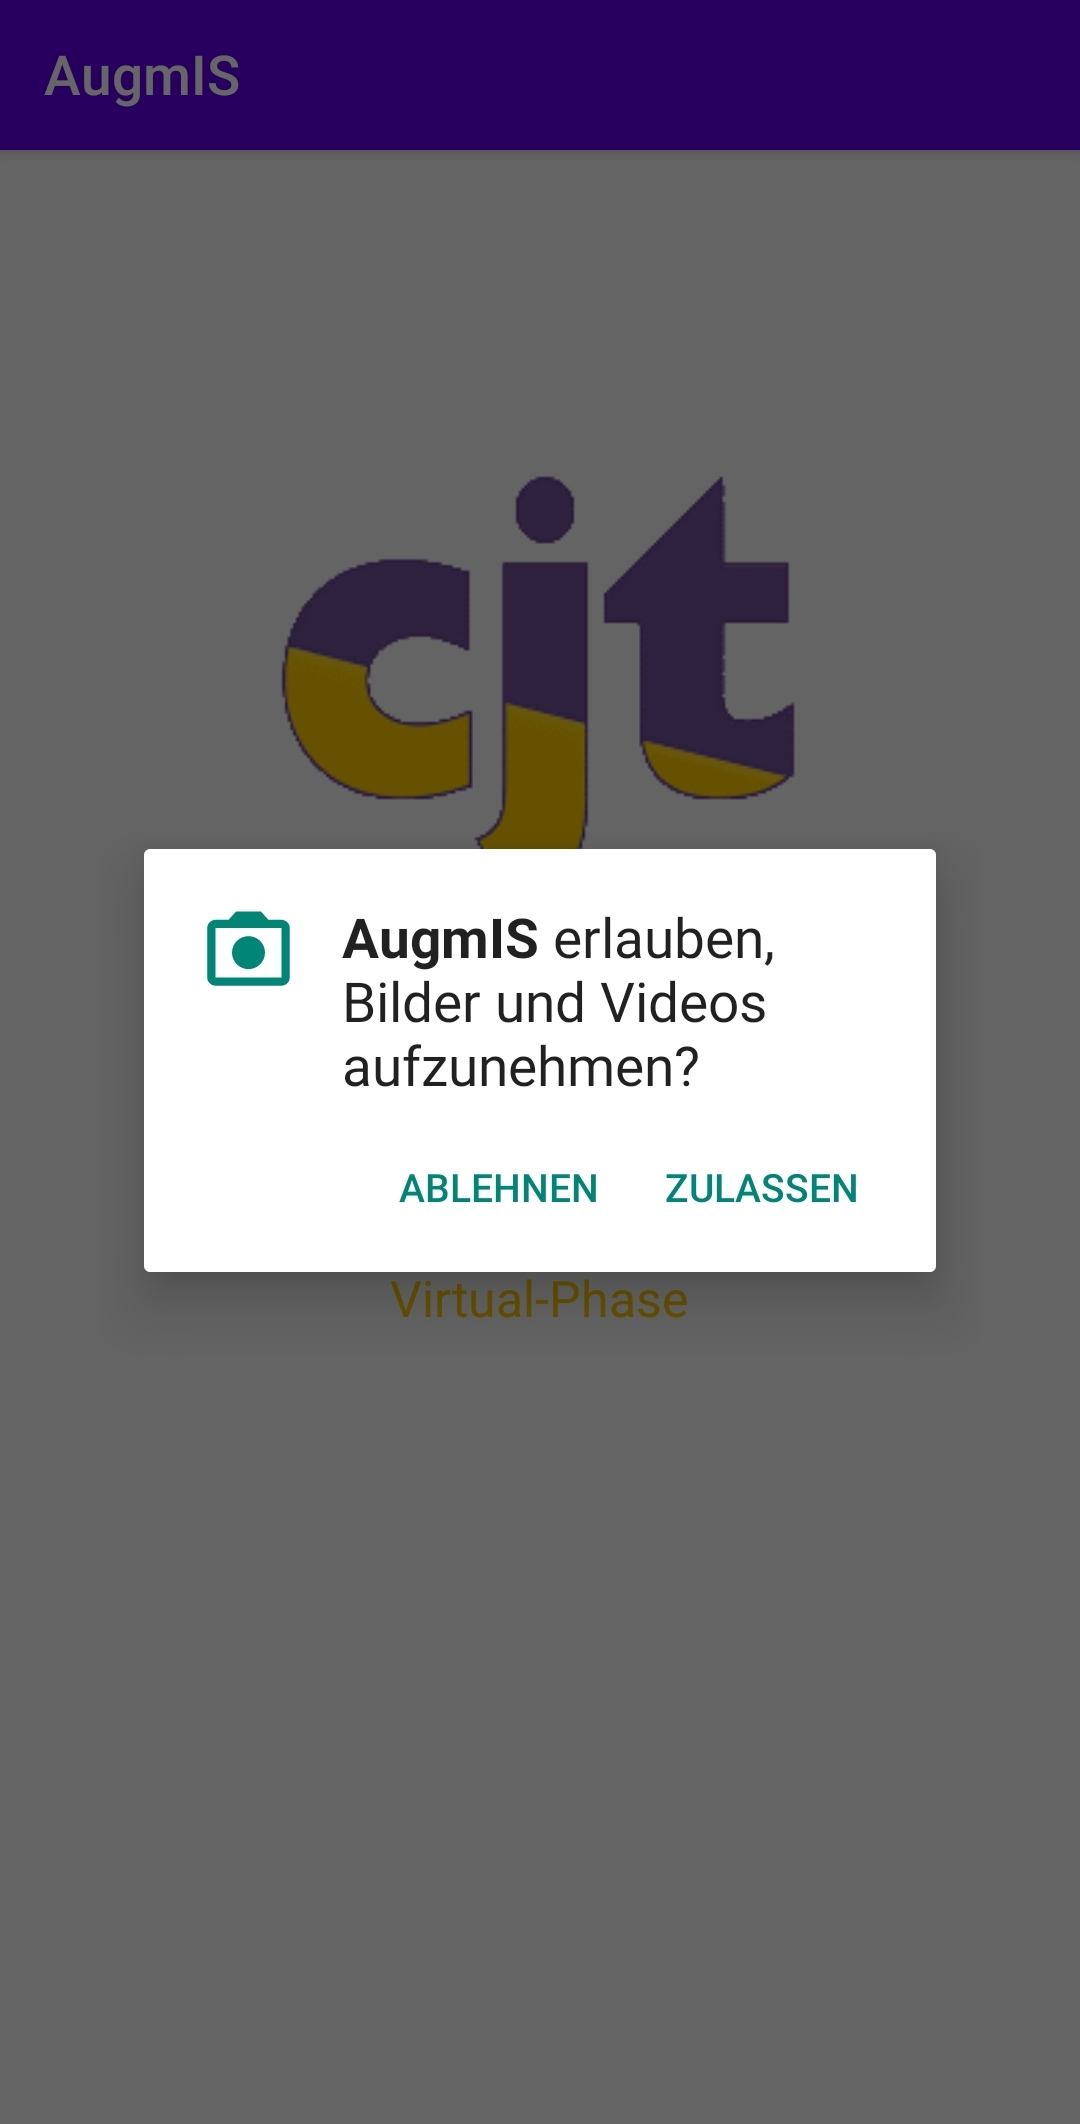
\includegraphics[width=10cm,height=7.5cm,keepaspectratio]{4Umsetzung/Bilder/camera_permission.jpg}
    \caption{Start der Applikation}
    \label{pic:camera_perm}
\end{figure}
\pagebreak
\\ 
Da speziell das Assistenzsystem auf die Hardware gegebene Komponente, die im Smart-Device integrierte Kamera, zugreift, zählt diese zu den nativen Applikationen. 
Darunter sind Anwendungen adressiert, die ausdrücklich für das Betriebssystem des Endgeräts konzipiert sind oder zum Beispiel auf die vom Endgerät vorhandenen Komponenten, 
zum Beispiel auf die Bild-Mediathek, Datei-Strukturen oder die oben bereits erwähnte Kamera Komponente, zugreifen.
\\ 
\linebreak
Angenommen der Nutzer lässt die Frage, die Kamera für das Assistenzsystem freizugeben, zu, dann startet die Applikation wie erwünscht. Darauf folgend ist letztendlich 
das eigentliche Startmenü zu sehen. Diese Ansicht ist der nachfolgenden Abbildung (\ref{pic:startmenu}) zu entnehmen. Ein sehr einfach und schlicht gehaltenes Design. 
Darauf ist zentriert das Firmen-Logo der cjt Systemsoftware AG zu sehen und lediglich zwei farblich voneinander getrennten Button zur Navigation innerhalb der Applikation. 
Die Button adressieren jeweils die nachfolgende, zugehörige Funktion. Zum einen 
zur Scan-Phase bei Betätigung des lilafarbenen Buttons und zum anderen zur Visualisierungs-Phase bei Bedienung des gelbfarbenen Buttons. In der Gesamtheit is das Layout 
ist an den Farben des Firmen-Logos angelehnt und bildet einen ruhigen und harmonischen Einstieg in das Programm. 
\\ 
Grundlegend wurden für die Designs der Benutzeroberflächen Prinzipien der \ac{UX}, berücksichtigt. Darunter folgende Punkte: 
\begin{itemize}
    \item Übersichtlichkeit (Digestibility): Auf einen Blick verstehen, worum es geht. Der User versteht intuitiv was zu tun ist.
    \item Klarheit (Clarity): Deutliche und verständliche Ausdrucksweise und klar herauszufindenden Nutzen der Funktion, bzw. Anwendung.
    \item Vertrauen (Trust): Gutes Design erlangt Vertrauen. Offenlegung der Aktionen und Hintergründe. 
    \item Begeisterung (Delight): Komplexe Sachverhalte einfach zu lösen. 
\end{itemize} 
\begin{figure}[hbt!]
    \centering
    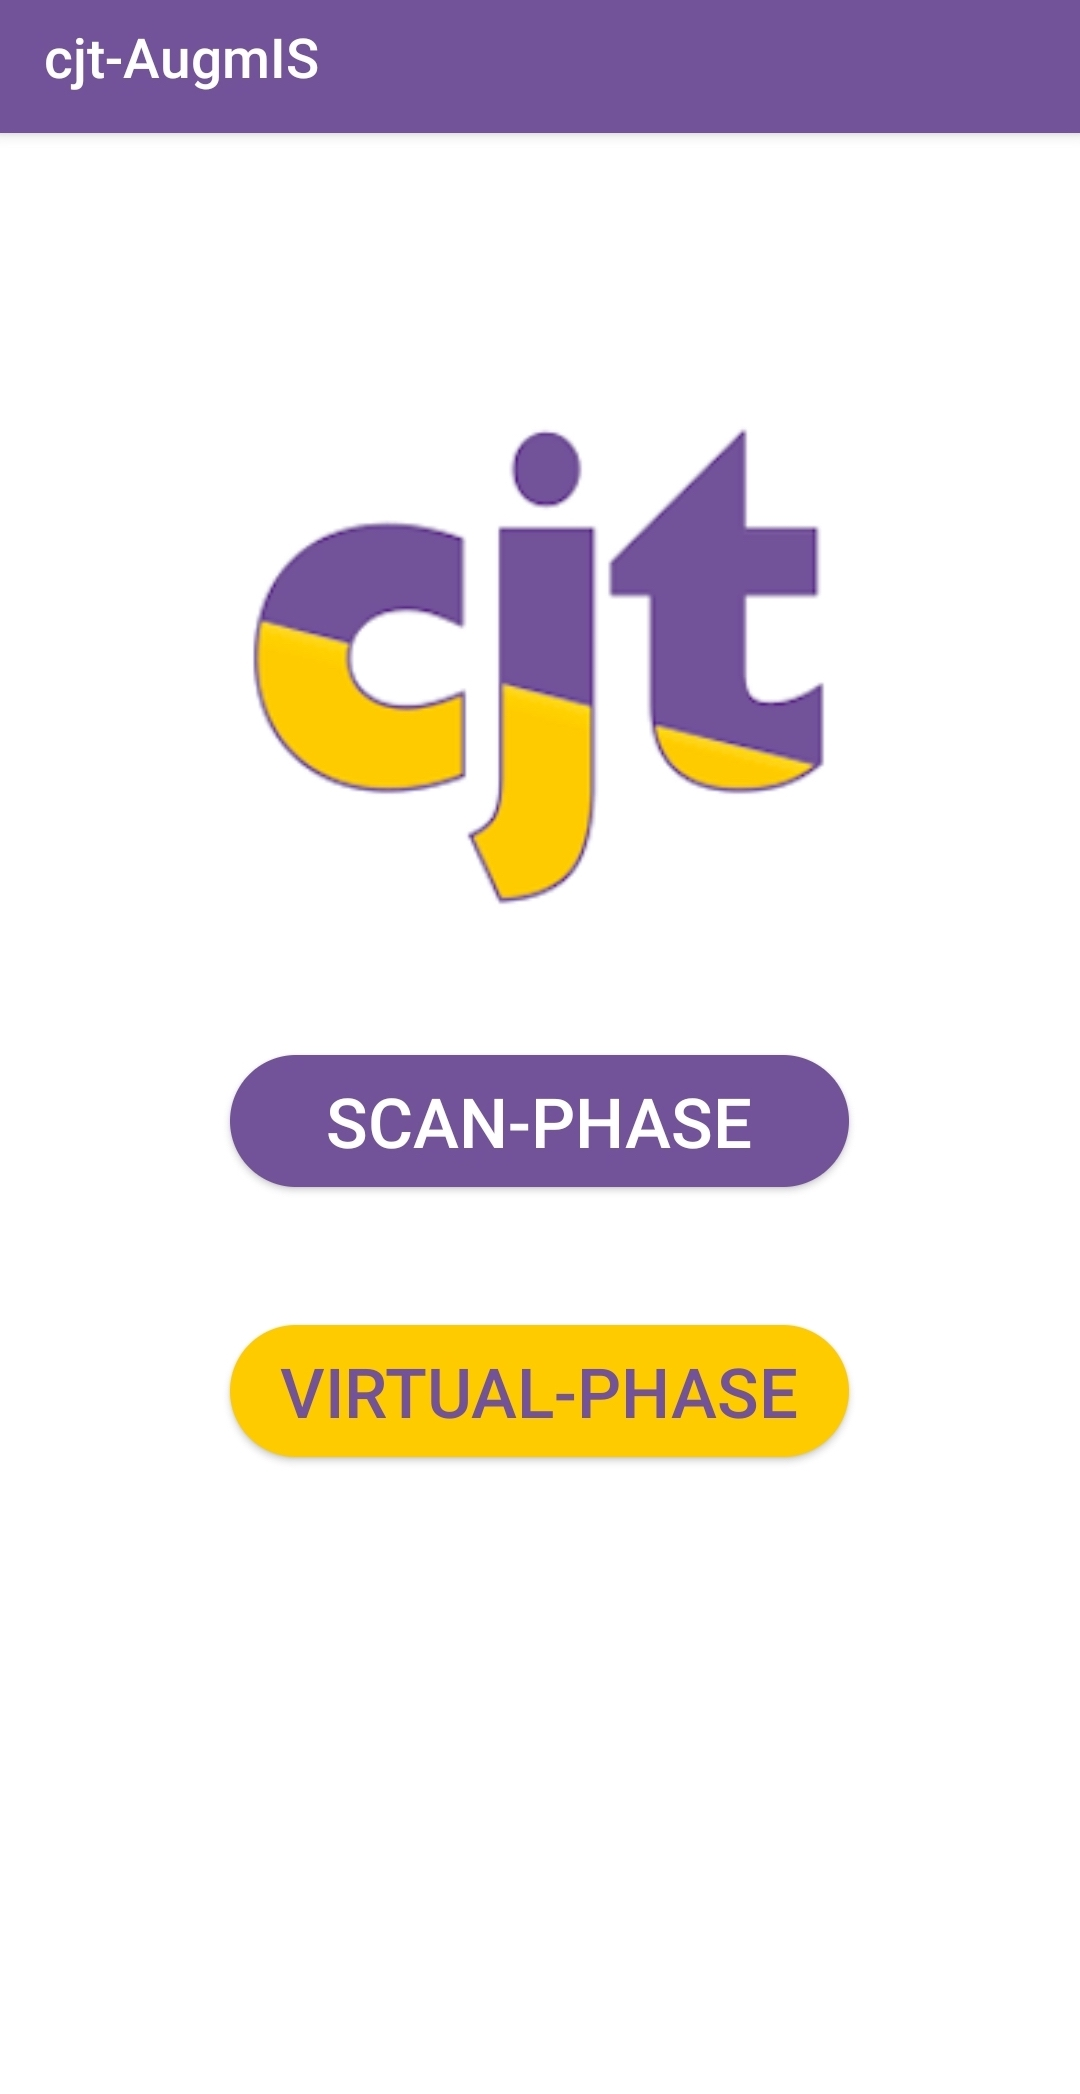
\includegraphics[width=10cm,height=7.5cm,keepaspectratio]{4Umsetzung/Bilder/startmenu.jpg}
    \caption{Startmenü der Applikation}
    \label{pic:startmenu}
\end{figure}
Nachdem das Design des Startmenüs und dem PopUp-Fenster abgeschlossen war, ging es darum, die Funktionalität der UI-Komponenten zu implementieren. 
\subsubsection{BackEnd}
Durch die schlicht und einfach gehaltene Modellierung des Startmenüs, zählt dieses als Ansicht zum Einstieg in die Nutzung des Assistenzsystems, zur Abfrage der 
\textit{„Camera-Permission“} und zur weiteren Navigation innerhalb der Anwendung.
\\ 
Mit der \textit{„Permission-Request“} wird abgefragt, ob die Genehmigung zur Nutzung der Kamera in der \textit{„AndroidManifest.xml“} erteilt wurde, bzw. wird dadurch 
das PopUp-Fenster zur Nachfrage der Genehmigung geöffnet und die daraus resultierende Antwort in die Manifest-Datei eingetragen. 
\\ 
\linebreak
Die Manifest-Datei beinhaltet alle optionalen Metadaten, im Bezug zum Assistenzsystem die für das Projekt benötigten Google ARCore-Metadaten, sowie grundlegende 
Informationen über das Projekt. Darunter welche Genehmigungen zur Ausführung der Applikation benötigt werden, welche Activities die Anwendung enthält und 
Stammdaten, z.B. Titel, -bild und App-Icon, die das Projekt eindeutig definieren.
\\ 
\linebreak
Demnach beinhaltet diese Funktion wenig Logik, bis auf die Abfrage der \textit{„Camera-Permission“} und die Button-Klick-Funktion, die den Nutzer jeweils auf die 
von ihm gewählte Funktion weiterleitet. Sozusagen eine simple Navigation.
\\ 
\linebreak
Als das Startmenü implementiert war, ging es an die Entwicklung der Scan-Phase, der ersten Kernfunktion des Assistenzsystems.  

\subsection{Scan-Phase} %Umgebungserkennung /
Bei der Implementierung der Scan-Phase kam es zu den ersten praktischen Berührpunkten mit der Google ARCore \acs{API}. Diese wurde zu Beginn studiert, 
um einen Überblick zu erlangen, wie die Struktur dieser Schnittstelle aufgebaut ist. Dadurch konnten Methoden und Funktionen analysiert werden, um im 
weiteren Verlauf der Entwicklung damit arbeiten zu können.
\subsubsection{FrontEnd}
\begin{figure}[hbt!]
    \centering
    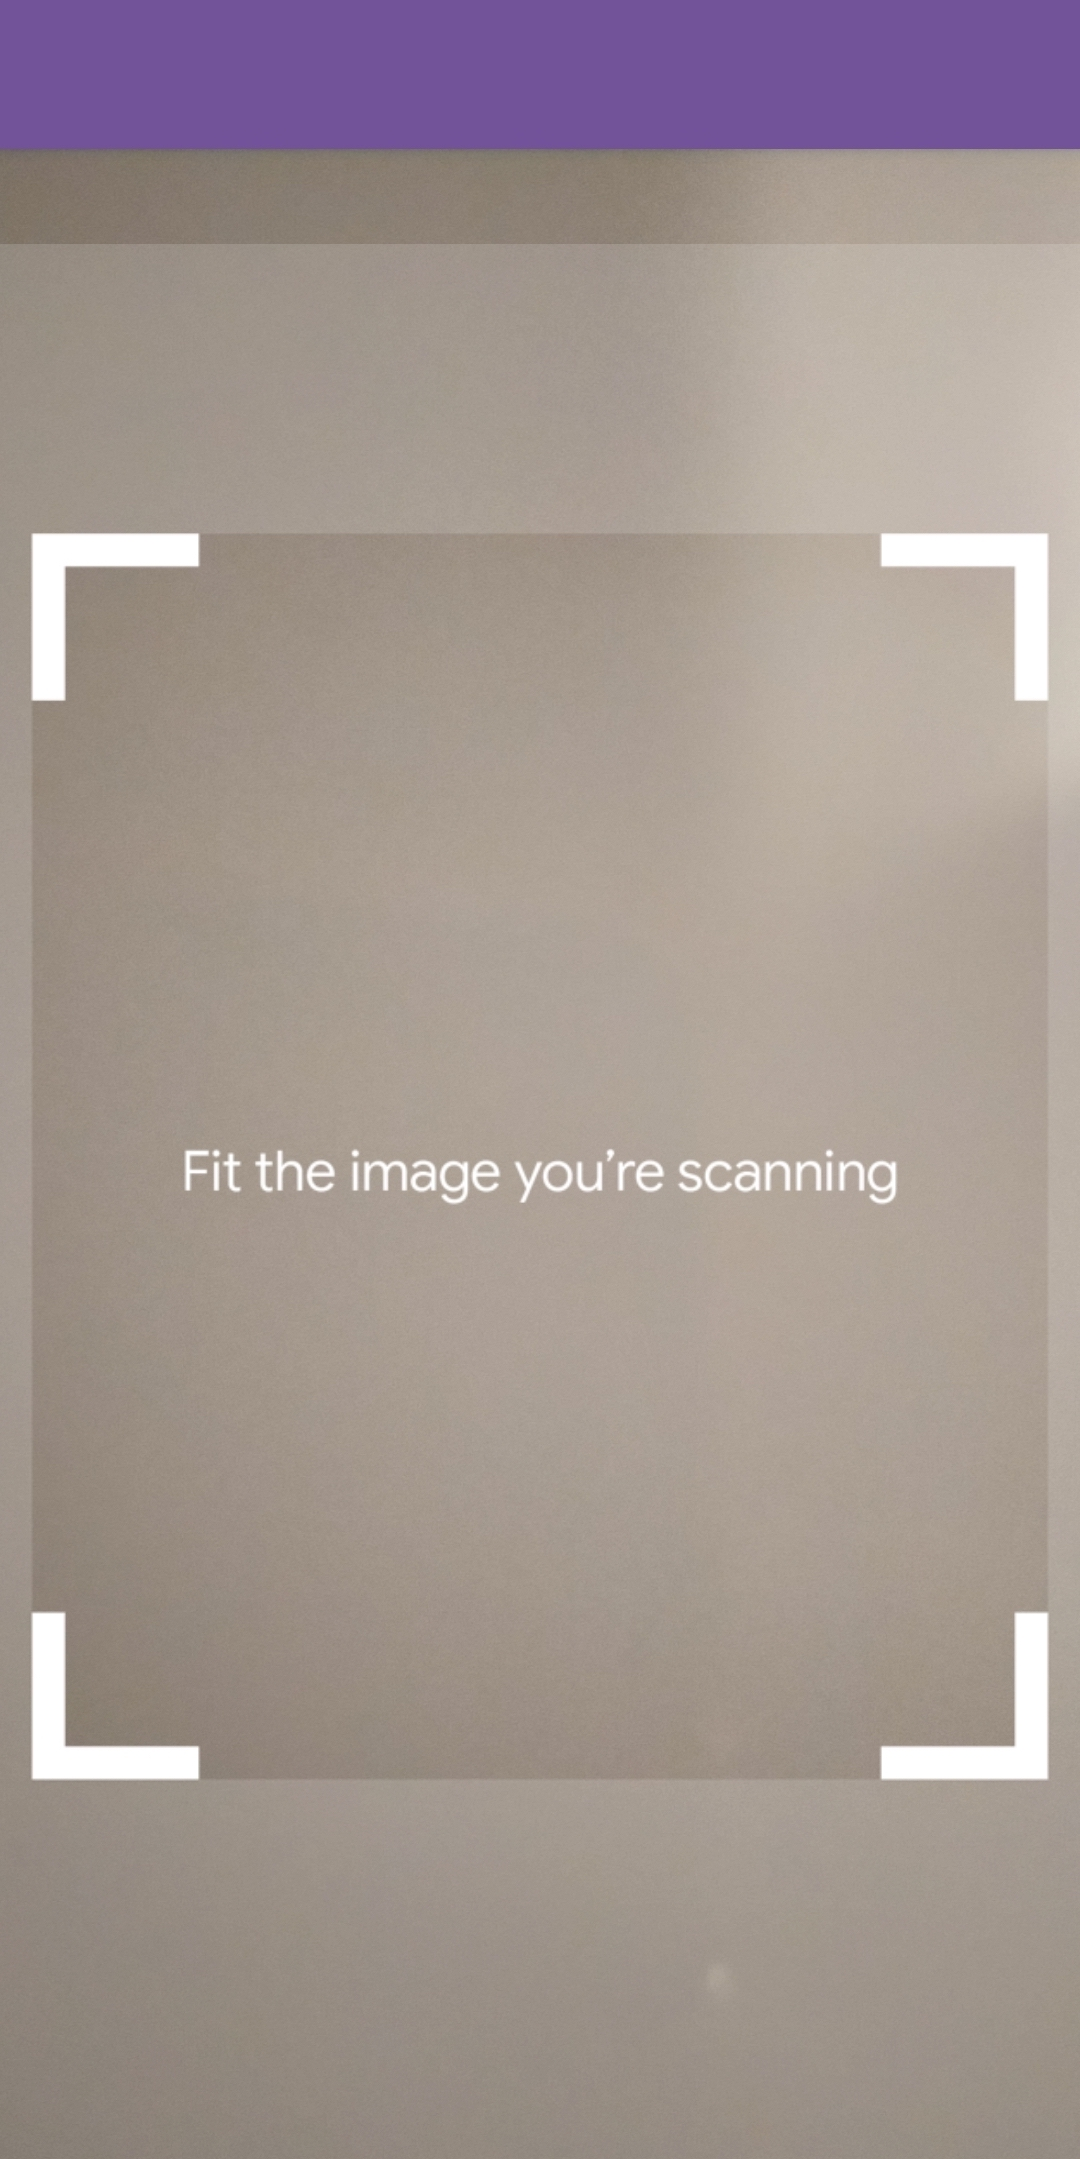
\includegraphics[width=10cm,height=7.5cm,keepaspectratio]{4Umsetzung/Bilder/image_tracking.jpg}
    \caption{Markererkennung der Applikation zum Start der Scan-Phase}
    \label{pic:image_tracking}
\end{figure}
\begin{figure}[hbt!]
    \centering
    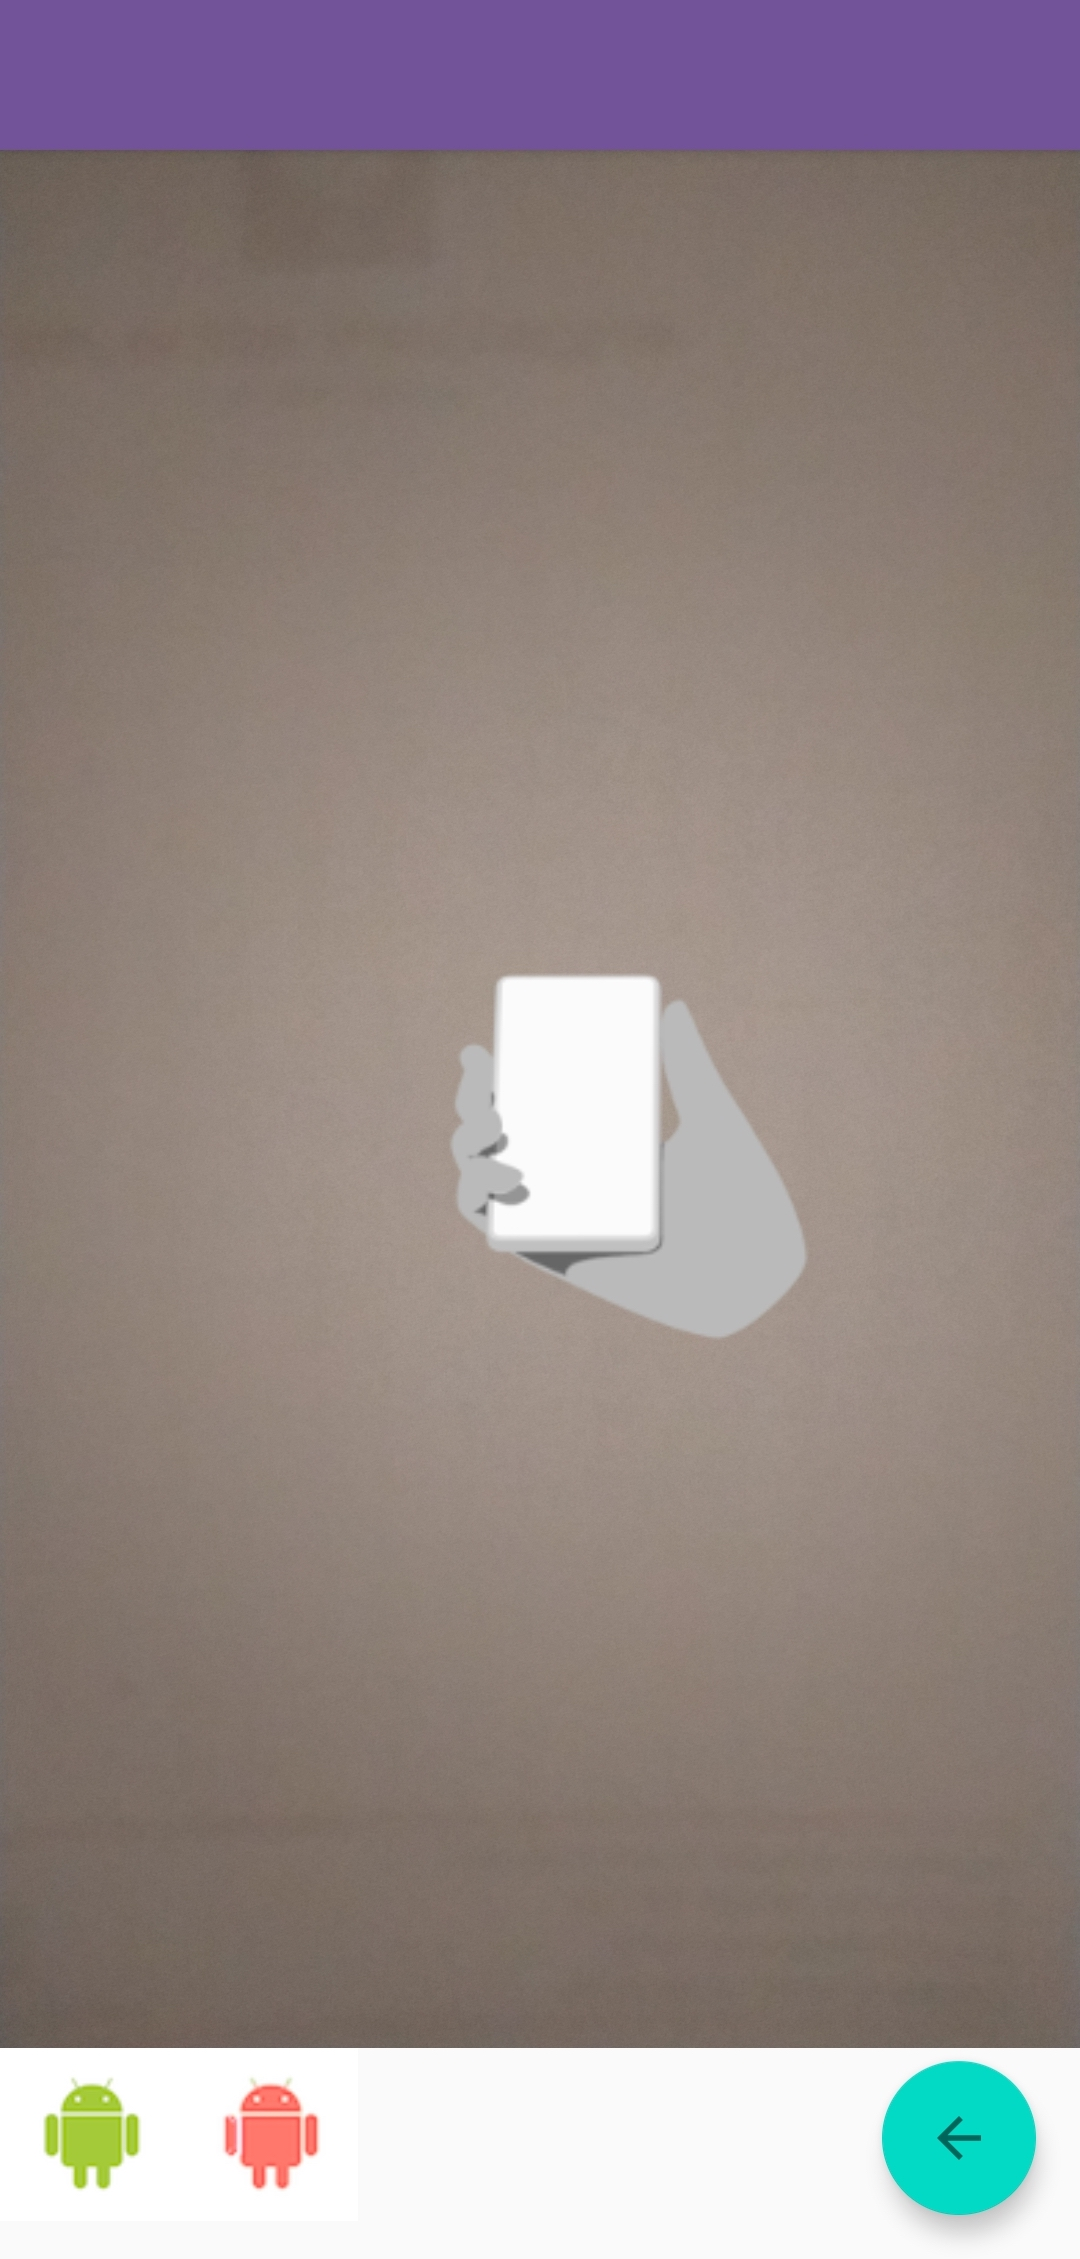
\includegraphics[width=10cm,height=7.5cm,keepaspectratio]{4Umsetzung/Bilder/scan-phase.jpg}
    \caption{Scan-Phase der Applikation}
    \label{pic:scan}
\end{figure}
\subsubsection{BackEnd}
\begin{figure}[hbt!]
    \centering
    
\includegraphics[width=5cm,height=5cm,keepaspectratio]{4Umsetzung/Bilder/cjt_logo_tracking.png}
    \caption{Marker zur Erkennung der Ausgangsposition}
    \label{pic:initialMarker}
\end{figure}

\subsection{Visualisierungs-Phase} 
\subsubsection{FrontEnd}
\begin{figure}[hbt!]
    \centering
    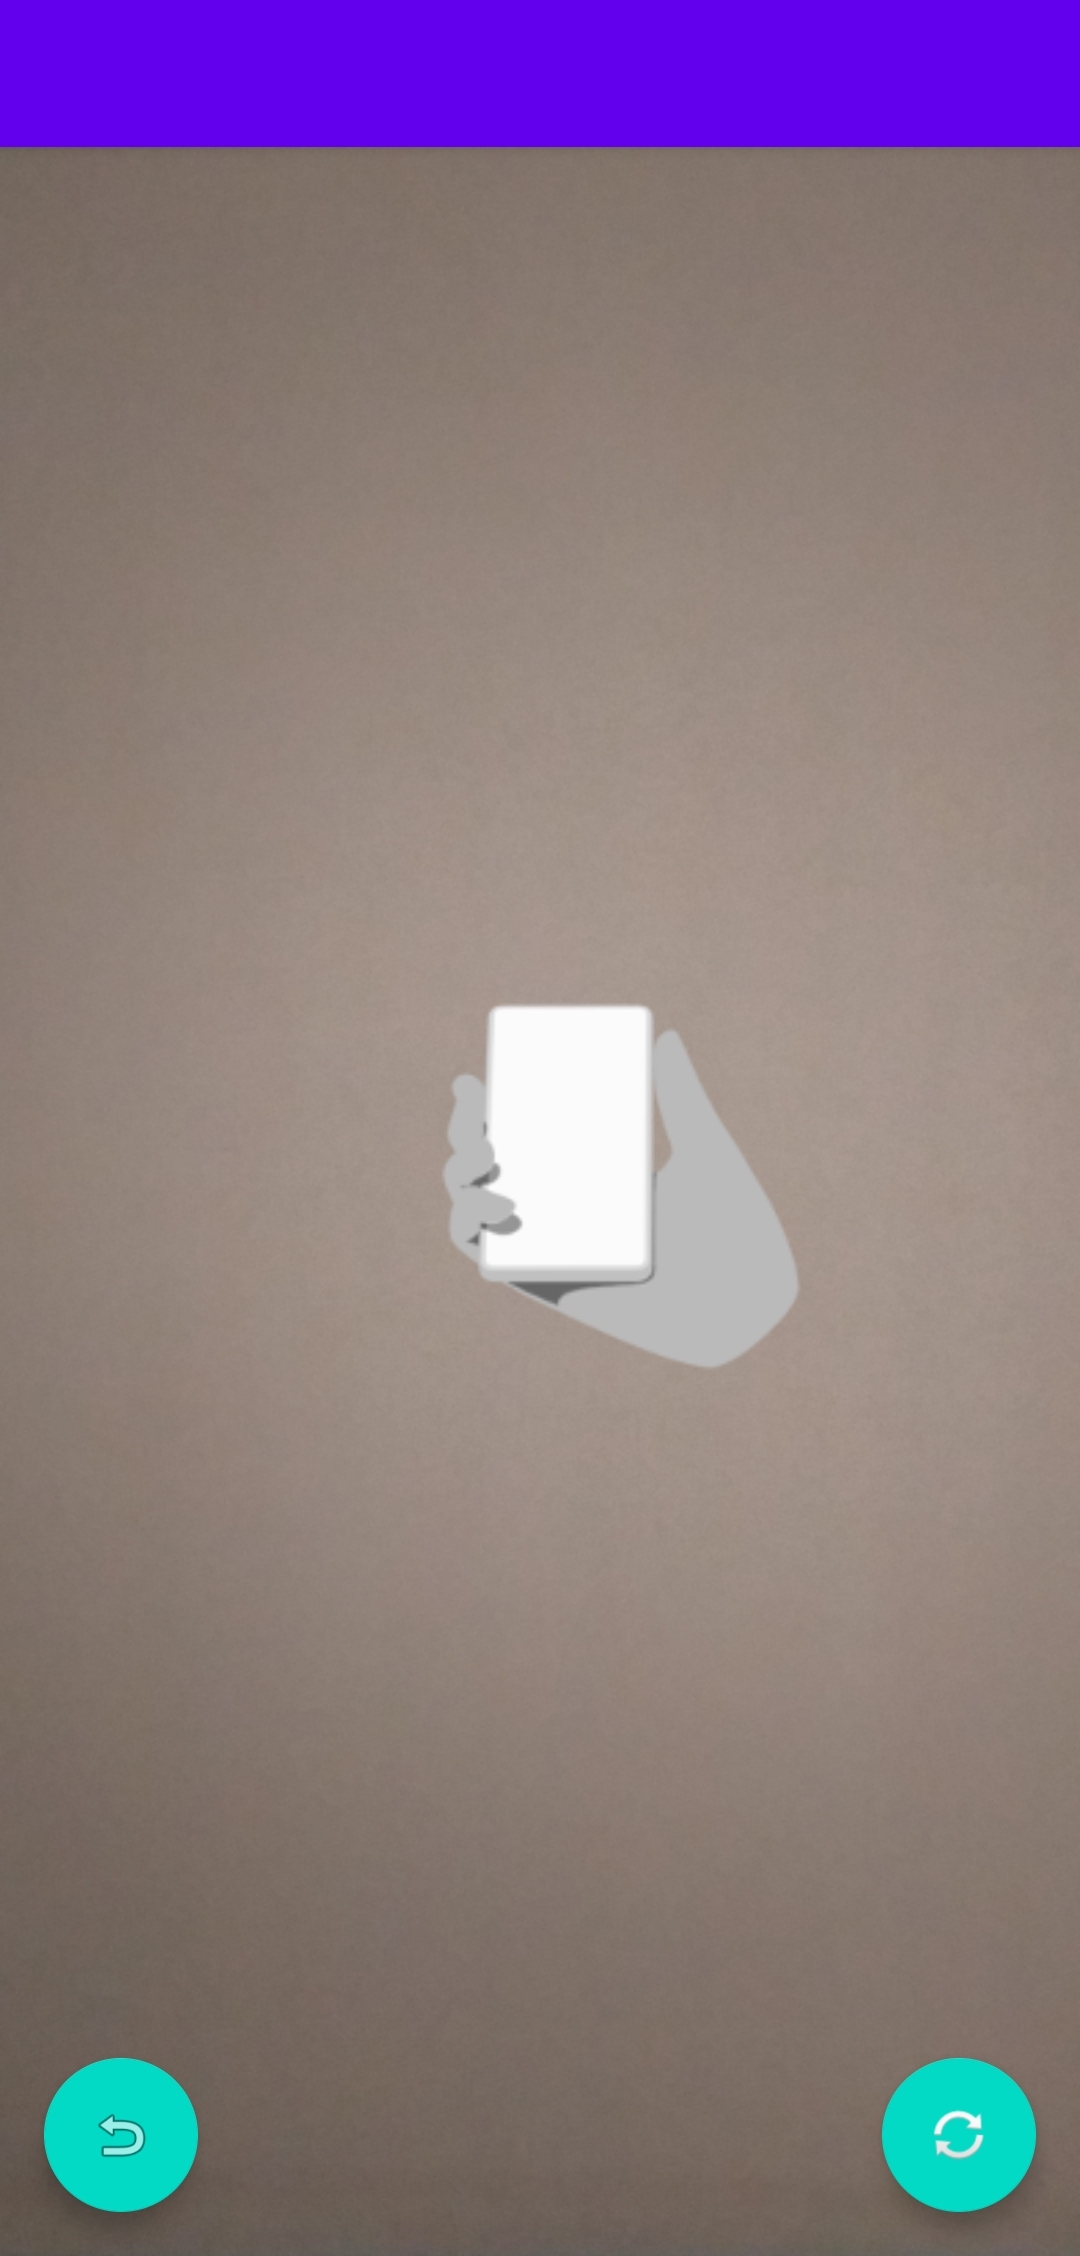
\includegraphics[width=10cm,height=7.5cm,keepaspectratio]{4Umsetzung/Bilder/visual-phase.jpg}
    \caption{Visualisierungs-Phase der Applikation}
    \label{pic:visual}
\end{figure}
\subsubsection{BackEnd}

\section{Testdurchlauf / Test-Szenario}
\label{chap:testdurchlauf}